\chapter{Общие вопросы}

В этой главе приводятся основные понятия ML и DS. 


\section{Машинное обучение}

Машинное обучение (ML) - область искусственного интеллекта, изучающая самообучающиеся модели, то есть решаюшие поставленную задачу не по заранее запрограммированному алгоритму, а предварительно настраивая свое поведение согласно имеющимся данным. 

Обычно методы ML содержат свободные параметры, подбор которых наилучшим (в смысле имеющихся данных и задачи) образом и составляет процесс обучения алгоритма. После обучения алгоритм можно использовать на новых данных, которые не были представлены алгоритму на стадии обучения.


\section{Эмпирический риск}

Будем считать, что обучающая выборка $(x_1, y_1)$, $(x_2, y_2)$, ... $(x_n, y_n)$ приходит из некоторого распределения с плотностью $f(x, y)$.
Пусть, далее, задано зависящее от параметра семейство алгоритмов $a = a(x, w)$ и некоторая функция потерь $L = L(y, a)$.

В этих условиях общая задача обучения с учителем может быть формализованна как задача минимизации риска, то есть средней ошибки
$$
l(w) \equiv \mathbb{E}L = \int L(y, a(x, w))f(x, y)dxdy,
$$
$$
w_{opt} = \argmin l(w).
$$

Само распределение $f$ обычно не известно, однако, при условии, что обучающая выборка пришла из этого распределения, интеграл можно приближенно заменить  средним и таким образом оценить среднюю ошибку через \textbf{\textit{эмпирический риск}}
$$
r_{emp}(w) = \frac{1}{n}\sum_{i=1}^nL(y_i, a(x_i, w)) \approx l(w).
$$

Таким образом, основную задачу обучения можно пытаться решать минимизацией эмпирического риска вместо полного.


\section{Основные классы задач}

\subsection{Обучение с учителем}

\subsection{Обучение без учителя}

\subsection{Частичное обучение}

\subsection{Обучение с подкреплением}


\section{Обнаружение аномалий}


\section{Контроль качества}

...оценка обобщающей способности...


\section{Недообучение}


\section{Переобучение}


\section{Регуляризация}


\section{Отбор признаков}


\section{Параметры алгоритма}


\section{Подбора метапараметров}


\section{Основные типы алгоритмов}


\section{Многоклассовая классификация}

В задачах многоклассовой классификации каждый объект $x$ требуется отнести к двум или более классам $1, 2, ..., K$.
Такого рода задачи могут решаться как алгоритмами, способными сразу работать с любым числов классов, так и сведением к нескольким задачам бинарной классификации.

Подходы к решению:

\begin{enumerate}
    \item Использовать алгоритмы, способные сразу выдавать вектор оценок принадлежности объекта к каждому классу (нейросети, ближайшие соседи и пр.).
    \item One-vs-All: Решить $K$ задач по отделению $i$-го класса от всех остальных. В качестве оценки принадлежности объекта классу $i$ следует выбрать ответ $i$-го алгоритма на этом объекте:
$$
p(i|x) = a_i(x).
$$
Плюс в небольшом числе обучаемых классификаторов. Минус в том, что обучающие выборки становятся несбалансированными.
    \item One-vs-One: Решить $K(K-1)/2$ задач бинарной классификации для каждой пары классов. В качестве оценки принадлежности объекта классу $i$ следует взять сумму оценок принадлежностей этому классу всех алгоритмов, отделяющих $i$-й класс от остальных:
$$
p(i|x) = \sum_{j \neq i}a_{ij}(x).
$$
Плюс в том, что обучающие выборки сохраняют сбалансированность. Минус в том, что число обучаемых классификаторов квадратично велико.
    \item Error-Correcting Output Code (ECOC): Закодировать каждый класс вектором из нулей и единиц некоторого размера $k$ ($k\geqslant\log_2K$). Кодирующие векторы следует выбирать так, чтобы они образовывали коды, исправляющие ошибки. Обучаем $k$ бинарных классификаторов. На этапе предсказания для объекта формируем $k$-мерный вектор и относим его к тому классу, расстояние Хэмминга до которого минимально. 
\end{enumerate}


\section{Дисбаланс классов}

...чем плохо... как бороться (over/undersampling/SMOTE)...


\section{Ансамбли алгоритмов}

\section{Метрики и функции потерь}

Метрика - величина, обычно диктуемая бизнесом, оптимизация (максимизация или минимизация) которой вполне очевидным образом свидетельствует об улучшении качества работы модели.

Функция потерь - величина, более удобная для оценки/оптимизации модели, уменьшение которой, вообще говоря, приводит к оптимизации метрики задачи.

Иными словами, улучшение метрики - конечная цель процесса обучения алгоритма, но достигается это зачастую оптимизацией именно некоторой функции потерь, с которой может быть удобнее работать.
Метрики и функции потерь - близкие понятия, когда речь идет об оценки качества алгоритма, и их довольно часто смешивают.

\textbf{Пример:} Пусть в задаче бинарной классификации основной метрикой является accuracy - доля правильных ответов. Эта метрика не дифференцируема, поэтому ее оптимизация напрямую методами гладкой оптимизации невозможна. В качестве функции потерь выберем MSE - среднеквадратичную ошибку. Это уже гладкая функция своих аргументов,и ее минимизация скорее всего приведет к увеличению доли правильных ответов, то есть к конечной цели. 

\section{Метрики бинарной классификации}

Пусть некоторый алгоритм $a$ решает задачу бинарной классификации с классами $0$ (негативный) и $1$ (позитивный).
Тестирование алгоритма $a$ проводится на $n$ объектах, ответы $y$ на которых известны. Пусть $TP$ и $TN$ - числа правильно классифицированных позитивных и негативных объектов соответственно. Аналогично, $FP$ и $FN$ - числа неправильно классифицированных позитивных и негативных объектов соответственно.

О качестве алгоритма $a$ можно судить по матрице ошибок:
\begin{center}
\begin{tabular}{ c c c }
     & y=1 & y=0 \\ 
 a=1 & TP  & FP \\  
 a=0 & FN  & TN    
\end{tabular}
\end{center}

Для оценки качества работы алгоритмов бинарной классификации обычно используются описанные далее основные метрики.

\subsection{Accuracy}

Точность (accuracy) - доля правильных ответов,

$$
accuracy = \frac{TP + TN}{n}.
$$

Проста в использовании и интерпретации, но плоха для несбалансированных выборок. Кроме того, не дифференцируема и потому не может быть использована напрямую в качестве функции потерь для алгоритмов гладкой оптимизации.

\subsection{Precision}

Точность (precision) - отношение числа правильно классифицированных позитивных объектов к общему количеству позитивно классифицированных,

$$
precision = \frac{TP}{TP + FP}.
$$

Чем ближе значение к 1, тем меньше ложных срабатываний (FP). Проста в использовании и интуитивна, то не использует информацию о негативно классифицированных объектах и, кроме того, не является дифференцируемой.

\subsection{Полнота (recall)}

Полнота (recall) - вычисляется как отношение

$$
recall = \frac{TP}{TP + FN}.
$$

Чем ближе значение к 1, тем меньше ложных пропусков (FN). Проста в использовании и интуитивна, то не использует TN, FP и, кроме того, не является дифференцируемой.

\subsection{F1-мера}

F1-мера - среднее гармоническое точности и полноты,

$$
F = \frac{2PR}{P + R}.
$$

F1-мера усредняет точность и полноту, является неплохом компромиссом между обеими метриками. Проста в использовании, но плохо интерпретируема и не является дифференцируемой.

\subsection{F-мера}

Обобщенная F-мера вычисляется как

$$
F = (1+\beta^2)\frac{PR}{\beta^2P + R}.
$$

F-мера усредняет точность и полноту, является неплохом компромиссом между обеими метриками, имеет настраиваемый параметр $\beta$. Проста в использовании, но плохо интерпретируема и не является дифференцируемой.

\subsection{ROC кривая}\label{roc-curve}

ROC кривая - характеристика качества алгоритмов бинарной классификации, дающих вероятностноподобный вывод, $a\in[0, 1]$. 
ROC кривая строится в координатах 
$$
FPR = \frac{FP}{FP + TN}, \quad TPR = \frac{TP}{TP + FN}.
$$
Каждая точка кривой - значение $(FPR, TPR)$, полученное для некоторого порога дискретизации алгоритма (см. \ref{pr-curve}). 

Более простой способ построения ROC кривой состоит в следующем:
\begin{enumerate}
    \item отрезки $[0, 1]$ по осям $TPR$ и $FPR$ разбиваются на $\#[y=0]$ и $\#[y=1]$ частей соответственно.
    \item пары реальных ответов $y_i$ упорядочиваются по убыванию соответствующих ответов алгоритма $a_i$.
    \item проходя по получившемуся после сортировки массиву значений $y_i$, строим ROC кривую, начиная от начала координат и делая шаг вправо, если $y_i=0$ и вверх, если $y_i=1$. Важный момент: если рядом по порядку оказались несколько $a_i$ с одинаковыми значениями, то соответствующий им участок ROC кривой будет не ступенчатым, а прямолинейным (см. пример ниже).
\end{enumerate}

ROC кривая идеального алгорима проходит через точки $(0,0)$, $(0,1)$, $(1,1)$; для случайного гадания - проходит вблизи прямой $FPR = TPR$. Наилучшим значением порога дискретизации алгоритма может считаться порог, соответствующий точке на ROC кривой, ближайшей к $(0, 1)$, либо точке, наиболее удаленной от прямой случайного гадания $TPR = FPR$. 

\textbf{Пример:} для алгоритма, дающего вывод как в таблице ниже, график $ROC$ кривой выглядит следующим образом

\begin{tabular}{ c c }
    \raisebox{-\totalheight}{
    \begin{tabular}{|c|c|c|c|c|c|c|c|} 
        \hline
        y & 1 & 0 & 0 & 1 & 0 & 1 & 0 \\ 
        \hline
        a & 1.0 & 0.9 & 0.9 & 0.9 & 0.8 & 0.3 & 0.2 \\
        \hline
    \end{tabular}}
    & 
    \raisebox{-\totalheight}{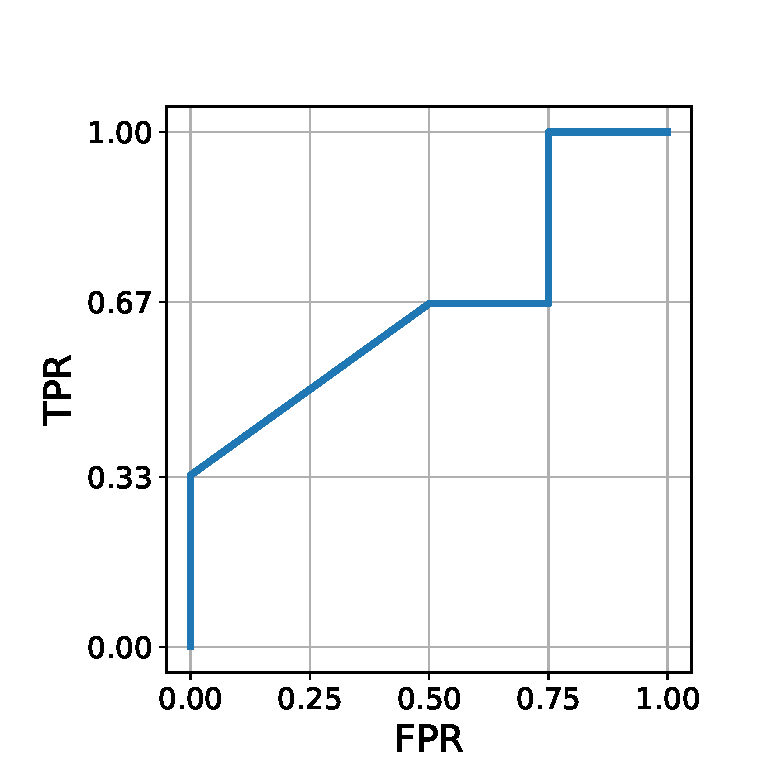
\includegraphics[scale=0.4]{images/roc-curve.eps}}
\end{tabular}

\subsection{ROC-AUC}

ROC-AUC - площадь под ROC кривой. Применяется к алгоритмам бинарной классификации, дающим вероятностноподобный вывод, $a\in[0, 1]$, позволяя оценить алгоритм "в целом", без привязки к конкретному значению порога дискретизации алгоритма.

ROC-AUC принимает значения от $0$ до $1$. Значения близкие к $0.5$ интерпретируются как самые худшие (случайное гадание), близкие к $1$ - как хорошие. ROC-AUC более устойчива к дисбалансу классов, чем Accuracy, но не так хорошо, как PR-AUC. ROC-AUC также не учитывает уверенность алгоритма в своих предсказаниях (насколько близко распределены предсказания к $0$ и $1$). Не является дифференцируемой.

ROC-AUC для примера \ref{roc-curve} равна $2/3$.

\subsection{PR кривая}\label{pr-curve}

PR кривая - характеристика качества алгоритмов бинарной классификации, дающих вероятностноподобный вывод, $a\in[0, 1]$. 
PR кривая строится в координатах 
$$
recall = \frac{TP}{TP + FN}, \quad precision = \frac{TP}{TP + FP}.
$$
Каждая точка кривой - значение $(recall, precision)$, полученное для некоторого порога дискретизации алгоритма. 

Способ построения PR кривой состоит в следующем:
\begin{enumerate}
    \item вычисляются пороги $h$ - всевозможные значения ответов алгоритма $a$.
    \item ответы $a_i$ дискретизируются для каждого значения порога и вычисляются значения $recall$ и $precision$. При этом ордината первой точки кривой, соответствующей порогу $h>1$, не определена, так как знаменатель $precision$ обращается в ноль. В качестве ординаты берется ордината второй точки.
    \item по полученным точкам строится график PR кривой. 
\end{enumerate}

PR кривая идеального алгорима проходит через точки $(0,1)$, $(1,1)$, $(1,\#[y=1]/n)$; для случайного гадания - проходит вблизи прямой $precision = \#[y=1]/n$.

\textbf{Пример:} для алгоритма, дающего вывод как в таблице ниже, график $PR$ кривой выглядит следующим образом

\begin{tabular}{ c c }
    \raisebox{-\totalheight}{
    \begin{tabular}{|c|c|c|c|c|c|c|c|} 
        \hline
        y & 1 & 0 & 0 & 1 & 0 & 1 & 0 \\ 
        \hline
        a & 1.0 & 0.9 & 0.9 & 0.9 & 0.8 & 0.3 & 0.2 \\
        \hline
    \end{tabular}}
    & 
    \raisebox{-\totalheight}{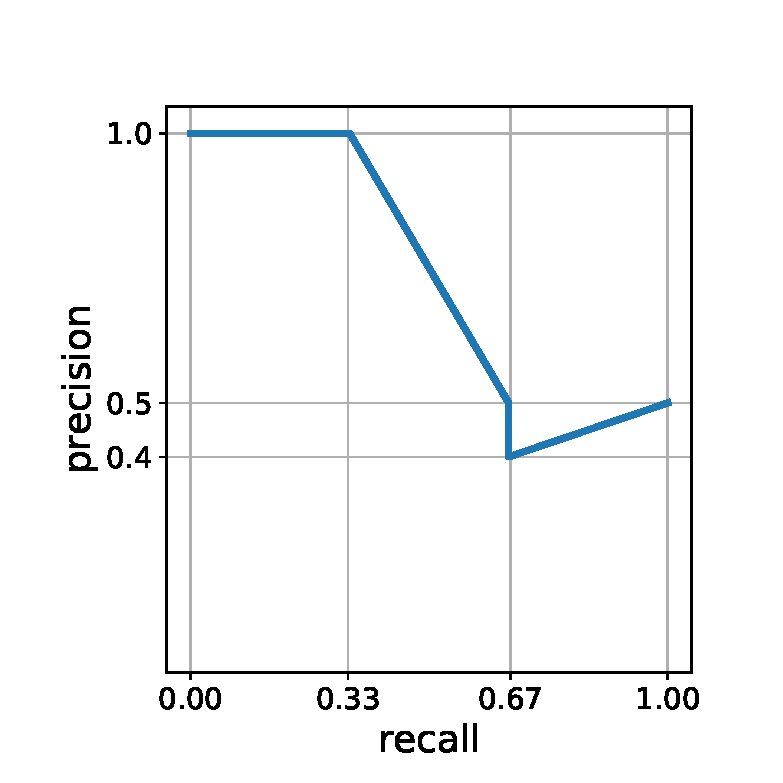
\includegraphics[scale=0.4]{images/pr-curve.eps}}
\end{tabular}

\subsection{PR-AUC}

PR-AUC - площадь под PR кривой. Применяется к алгоритмам бинарной классификации, дающим вероятностноподобный вывод, $a\in[0, 1]$, позволяя оценить алгоритм "в целом", без привязки к конкретному значению порога дискретизации алгоритма.

PR-AUC - площадь под PR кривой. Принимает значения от $0$ до $1$. Значения близкие к $1$ интерпретируются как хорошие, близкие к $\#[y=1]/n$ - как самые худшие (случайные гадания). PR-AUC более устойчива к дисбалансу классов, чем ROC-AUC, однако, не учитывает уверенность алгоритма в своих предсказаниях (насколько близко распределены предсказания к $0$ и $1$). Не является дифференцируемой.

PR-AUC для примера \ref{pr-curve} равна $11/15\approx 0.73$.

\subsection{Бинарная кросс-энтропия (logloss)}

Пусть $y$ - истинная метка объекта ($0$ или $1$), а $a$ - ответы некоторого алгоритма (число из $[0, 1]$). Бинарная кросс-энтропия (logloss) вычисляется как
$$
L(y, a) = -y\log_2 a - (1-y)\log_2(1-a).
$$
Слагаемые с нулевым множителем при логарифме (соответствующие $y=0$ и $y=1$) полагаются равными нулю.

Полная кросс-энтропия на множестве ответов определяется усреднением значений по всем объектам.

Бинарная кросс-энтропия имеет следующую вероятностную интерпретацию. Пусть метка $i$-му объекту назначается по схеме Бернулли, т.е. метка полагается равной $y_i=1$ с вероятностью $a_i$ и $y_i=0$ с вероятностью $1-a_i$. Тогда вероятность получить истинные ответы $y_i$ равна
$$
\prod_{i=1}^na_i^{y_i}(1-a_i)^{1-y_i}.
$$
Логарифмируя, получаем правдоподобие, совпадающее с бинарной кросс-энтропией с точностью до знака. Таким образом, нахождение ответов $a_i$ с позиции минимизации бинарной кросс-энтропии равносильно максимизации правдоподобия.


https://en.wikipedia.org/wiki/Loss_functions_for_classification


\section{Метрики многоклассовой классификации}

\subsection{Категориальная кросс-энтропия (logloss)}


\section{Индекс Джини}


\section{Метрики регрессии}

\subsection{Среднеквадратичная ошибка (MSE)}

Пусть $y$ - истинная метка объекта, а $a$ - ответы некоторого алгоритма. Квадратичная ошибка вычисляется как
$$
L(y, a) = (y - a)^2.
$$

Полная cреднеквадратичная ошибка на множестве ответов определяется усреднением значений по всем объектам.
Наилучшим константным предсказанием для MSE является выборочное среднее:
$$
a = \frac{1}{n}\sum_{i=1}^ny_i
$$

MSE дифференцируема и проста в использовании, но плохо интрепретируема, так как дает ненормированный ни к чему результат, который трудно с чем-либо сравнить. Кроме того, MSE чувствительна к выбросам в выборке.

\subsection{Среднеабсолютная ошибка (MAE)}

Пусть $y$ - истинная метка объекта, а $a$ - ответы некоторого алгоритма. Абсолютная ошибка вычисляется как
$$
L(y, a) = |y - a|.
$$

Полная cреднеквадратичная ошибка на множестве ответов определяется усреднением значений по всем объектам.
Наилучшим константным предсказанием для MSE является выборочная медиана.

MAE проста в использовании, но недифференцируема и плохо интрепретируема, так как дает ненормированный ни к чему результат, который трудно с чем-либо сравнить. MAE менее чувствительна к выбросам в выборке, чем MSE.


\subsection{Коэффициент детерминации ($R^2$)}

Пусть $y_i$ - истинные метки объектов $x_i$, а $a_i$ - ответы некоторого алгоритма. Коэффициент детерминации $R^2$ вычисляется как
$$
R^2(y, a) = 1 - \frac{\sum_{i=1}^n(y_i - a_i)^2}{\sum_{i=1}^n(y_i - \hat{y})^2}, \quad \hat{y} = \frac{1}{n}\sum_{i=1}^ny_i.
$$

$R^2$ показывает долю дисперсии $y_i$, объясняемую моделью. Является по сути линейной функцией от MSE, но более интерпретируема в силу нормировки к результату с константным прогнозом $\hat{y}$. Минусом является увеличение $R^2$ при увеличении числа признаков, что далеко не всегда свидетельствует о увеличении качества модели.


\section{Метрики кластеризации}


\section{Разложение ошибки алгоритма}

Будем считать, что обучающая выборка $X = (x_1, y_1)$, $(x_2, y_2)$, ... $(x_n, y_n) \in (\mathbb{X}\times\mathbb{Y})^n$ приходит из некоторого распределения с плотностью $f(x, y)$. Пусть также задан метод обучения $\mu: (\mathbb{X}\times\mathbb{Y})^n \rightarrow A$, который произвольной обучающей выборке ставит в соответствие алгоритм из некоторого семейства $A$. Будем использовать квадратичную функцию потерь, $L(y, a) = (y - a)^2$.

Мерой качества метода обучения $\mu$ естесственно считать усредненный по всевозможным обучающим выборкам средний риск:
$$
L(\mu) = \mathbb{E}_X\left[\mathbb{E}_{x,y}\left(y - \mu(X)(x)\right)^2 \right]
$$
Можно показать, что эта величина раскладывается в сумму трех:
$$
L(\mu) = \underbrace{\mathbb{E}_{x,y}\left(y - a_{*}(x)\right)^2}_\text{шум} +
         \underbrace{\mathbb{E}_x\left(\mathbb{E}_X\mu(X)(x) - a_{*}(x)\right)^2}_\text{смещение} +
         \underbrace{\mathbb{E}_x\left[\mathbb{D}_X\mu(X)(x)\right]}_\text{разброс},
$$
где $a_{*}(x) = \mathbb{E}_y\left[y|x\right]$ - наилучший из теоретически возможных алгоритм для среднеквадратичной функции потерь. 

\begin{enumerate}
    \item Шум (noise) - ошибка идеального алгоритма, невозможно как-либо уменьшить.
    \item Смещение (bias) - отклонение среднего ответа обученного алгоритма от ответа идеального. Показывает, насколько хорошо можно приблизить идеальный алгоритм с помощью имеющихся данных. Смещение, как правило, маленькое у сложных семейств (деревьев) и велико у простых (линейных).
    \item Дисперсия (variance) - разброс ответов обученных алгоритмов относительно их средних ответов. Показывает, насколько сильно может меняться ответ при варьировании выборки. Дисперсия, как правило, мала у простых алгоритмов и велика у сложных.
\end{enumerate}

Таким образом, усложнением алгоритма можно добиться меньшего смещения, но при этом может существенно увеличиться разброс, что по сути является переобучением модели.

\section{Кривые валидации}


\section{Кривые обучения}


\section{Метрические методы}


\section{Метод ближайших соседей}


\section{Линейные методы}


\section{Линейная регрессия}


\section{Логистическая регрессия}

...отличие от линейной...


\section{SVM}


\section{Ядра и спрямляющие пространства}


\section{Решаюшие деревья}

Решающее дерево - бинарное дерево, во внутренних вершинах которого стоят предикаты $\beta: X \rightarrow \{0, 1\}$, а в листовых вершинах - элементы множества ответов $Y$ (классы для задач классификации и числа для регрессии).

В качестве предикатов обычно используются простые линейные индикаторы $\beta_{jt}(x) = [x^j < t]$ ($j$-й признак меньше порога $t$).

Базовый алгоритм построения дерева решений (ID3 алгоритм):

\begin{enumerate}
    \item Начинаем со всей обучающей выборки $U = x_{(1)}, ..., x_{(n)}$.
    \item Проверяем, не выполнился ли для текущей вершины некоторый критерий останова (максимальное число листьев, минимальное число объектов в вершине, все объекты одного класса и пр.). Если это так, то объявляем вершину листовой, помещая в нее в качестве предсказания наиболее многочисленный класс (для задачи классификации), либо среднее из ответов (для регрессии).
    \item Если критерий останова не выполнился, вершина объявляется внутренней. В нее помещается выбираем предикат, максимизирующий функционал качества
$$
(j,t) = \argmax Q(U, j, t), \quad Q(U, j, t) = H(U) - \frac{|U_l|}{|U|}H(U_l) - \frac{|U_r|}{|U|}H(U_r),
$$
где $U_l$, $U_r$ - подмножества выборки $U$, удовлетворяюшие и не удовлетворяющие предикату $\beta_{jt}$ соответственно, $H$ - некоторый критерий информативности (см. ниже). Информативность стремимся минимизировать, функционал качества, соответственно - максимизировать.
    \item Строим левое и правое поддерево, рекурсивно повторяя шаги 2-4 для подвыборок $U_l$, $U_r$.
\end{enumerate}

Приведенный алгоритм - жадный, так как на каждом шаге он старается максимизировать функционал качества, не заботясь о том, будет ли это оптимальным выбором в целом.

Пусть $p_k$ - доля объектов класса $k$ в выборке $U$ (части обучающей выборки, попавшей в любую вершину). Примеры критериев информативности:
\begin{enumerate}
    \item $H(U) = 1 - \max_k p_k$ - ошибка классификации,
    \item $H(U) = \sum_{k=1}^Kp_k(1 - p_k)$ - критерий Джини,
    \item $H(U) = -\sum_{k=1}^Kp_k\log p_k$ - энтропийный критерий.
\end{enumerate}
Достоинства решающих деревьев:
\begin{itemize}
    \item хорошая интерпретируемость,
    \item допускаются пропуски в данных,
    \item высокая скорость обучения и работы.
\end{itemize}
Недостатки:
\begin{itemize}
    \item склонность к переобучению,
    \item низкая статистическая значимость глубоких деревьев (выборка все меньше дальше от корня),
    \item чувствительность к шуму и выбору критерия инормативности.
\end{itemize}
С переобучением решающих деревьев обычно борятся стрижкой (pruning), либо объединением древьев в ансамбли - случайный лес.


\section{Случайный лес}

Случайный лес - алгоритм, строящийся на основе беггинга над решающими деревьями. Каждое дерево обучается по выборке, полученной бутстрапированием обучающей выборки и, кроме того, в каждой вершине разбиение ищется по некоторому подмножеству признаков. Таким образом достигается низкая коррелированность базовых алгоритмов, а следовательно, уменьшение разброса итогового ансамбля. Следует отметить, что случайное подмножество признаков выбирается свое для каждой вершины каждого дерева, а не одно на каждое дерево.

Каждое дерево в случайном лесе обучается по своей бутстрап-подвыборке, что дает возможность автоматически сделать out-of-bag оценку качества ансамбля, так как бутстрап в среднем использует только 63\% объектов:
$$
OOB = \frac{1}{n}\sum_{i=1}^nL(y_i, r(x_i)),
$$
где $r(x_i)$ - усредненный ответ для всех деревьев, которые не видели объект $x_i$ на этапе обучения, $L$ - некоторая функция потерь.


\section{Ансамбли алгоритмов}

\subsection{Идея ансаблирования}

Ансамблем алгоритмов называется алгоритм, использующий в своей работе другие (базовые) алгоритмы.
Простейший пример ансамбля в задачах классификации - комитет большинства:
$$
a(x) = \mode(a_1(x), ..., a_n(x)).
$$

Простейший пример ансамбля в регрессии - среднее ответов некоторых алгоритмов:
$$
a(x) = \frac{1}{n}\sum_{j=1}^na_i(x).
$$

Если алгоритмы $a_i$ независимы как случайные величины (функции случайной величины $x$ - объекта предсказания), имеют одинаковые средние и ограниченные одним числом $d$ дисперсии, то ансамбль $a$ будет иметь то же среднее и меньшую дисперсию:
$$
\mathbb{E}a = \mathbb{E}a_j, \quad \mathbb{D}a \leqslant \frac{d}{n}.
$$
Таким образом, независимые алгоритмы в среднем подавляют ошибки друг друга, уменьшая тем самым разброс значений.

Более сложные примеры ансамблей обычно включают в себя обучение базовых алгоритмов на различных подвыборках исходной обучающей выборки, своем подмножестве признаков и др. Также при ансамблировании алгоритмов следует учитывать возможное переобучение, связанное с тем, что мы в итоге настраиваем результирующий алгоритм, используя информацию обо всей обучающей выборке. Для оценки качества ансамбля лучше сохранять некоторую валидирующую часть обучающей выборки, невидимую для всех базовых алгоритмах на этапе их обучения.   

\subsection{Беггинг}

\subsection{Метод случайных подпространств}


\section{Градиентный бустинг}


\section{Байесовские методы}



